%! TEX root = ./main.tex
\chapter{星系与天体}

\label{chap:spheres}

\section*{单位设定}

游戏中的单位换算关系如表\ref{tbl:unit-conversion}所列,功率、能量、时间等其他单位的换算关系与SI单位制相同:

\begin{table}[h]
    \centering
    \small
    \caption{单位换算关系}
    \begin{tabular}{ccc}
        \toprule
        单位描述 & 单位符号 & 换算关系 \\
        \midrule
        行星单位直径 & $D$ & $400\mathrm m$ \\
        恒星单位半径 & $R\odot$ & $1600\mathrm m$ \\
        天文单位 & AU & $40000\mathrm m$ \\
        光年 & LY & $60\mathrm {AU}$ \\
        \bottomrule
    \end{tabular}
    \label{tbl:unit-conversion}
\end{table}

\section{恒星}

在“新游戏”界面,玩家可以手动选择星系种子,恒星数量与星球资源倍率。星系种子、恒星数量决定了星区中恒星的分布。在游戏中,恒星的参数有质量、光谱类型、半径、光度、表面温度及年龄等。\index{恒星}\index{星系种子}

\subsection{光谱类型}

\index{光谱类型}

恒星共有M、K、G、F、A、B、O等光谱类型,其光度按照此顺序递增。同时,恒星颜色从红色逐渐过渡到黄色、白色直至蓝色(图\ref{fig:color-dist})。此外,白矮星、黑洞、中子星在游戏中同样被视为恒星,它们在游戏内的光谱类型显示为X。除普通恒星外,星系中会少量分布巨星恒星,它们相较于普通恒星有更大的质量和半径。以红巨星、蓝巨星最为常见,黄巨星及白巨星出现的频率较少。红巨星可能的光谱类型包含M、K、G等,蓝巨星可能的光谱类型包含A、B、O等。
\index{白矮星}\index{黑洞}\index{中子星}\index{巨星}

\begin{figure}[htb]
    \centering
    \subfigure[M]{\starimg M}
    \subfigure[K]{\starimg K}
    \subfigure[G]{\starimg G}
    \subfigure[F]{\starimg F}
    \subfigure[A]{\starimg A}
    \subfigure[B]{\starimg B}
    \subfigure[O]{\starimg O}
    \caption{不同光谱类型的恒星}
    \label{fig:color-dist}
\end{figure}

不同光谱类型的恒星在星系中的出现频率不同,B型恒星与G型恒星在星系中出现最为频繁。表\ref{tbl:amount-dist}统计了100个随机星系种子中不同类型恒星的数量分布(恒星数量固定为64)。

\begin{table}[h]
    \centering
    \small
    \caption{恒星数量分布}
    \begin{tabular}{ccccc}
        \toprule
        光谱类型 & 恒星平均数量 & 百分比 & 方差 & $95\%$置信区间 \\
        \midrule
        M & $4.84$ & $7.6\%$ & $3.20$ & $(4.49, 5.19)$ \\
        K & $10.2$ & $16.0\%$ & $6.80$ & $(9.72, 10.7)$ \\
        G & $13.8$ & $21.5\%$ & $7.05$ & $(13.2, 14.3)$ \\
        F & $4.90$ & $7.7\%$ & $2.78$ & $(4.57, 5.23)$ \\
        A & $2.99$ & $4.7\%$ & $2.68$ & $(2.67, 3.31)$ \\
        B & $21.1$ & $33.0\%$ & $2.66$ & $(20.8, 21.6)$ \\
        O & $2.12$ & $3.3\%$ & $1.15$ & $(1.91, 2.33)$ \\
        X & $4.00$ & $6.2\%$ & $0.00$ & $(4.00, 4.00)$ \\
        \bottomrule
    \end{tabular}
    \label{tbl:amount-dist}
\end{table}

恒星的光谱类型决定了其质量、光度及半径分布。除巨星外,O型恒星有最高的质量、最高的光度和最大的半径,M型恒星的质量和半径最小,光度最低。因此,在玩家选择建设戴森球(参见第\ref{chap:dyson-sphere}章)时,通常会选择在O型恒星、B型恒星或蓝巨星的行星上建立戴森球。它们更大的半径意味着可以建立更大的戴森球,更高的光度意味着单位面积戴森球壳可以接收到更多的能量。

\section{行星}

\index{行星}

行星是围绕恒星或巨行星运转的星球。每颗恒星的行星系都会包含1-6颗行星。其中气态巨星或冰巨星也会伴随若干颗卫星生成。

\subsection{类型}

\index{行星!类型}

行星的不同类型会影响其资源分布,游戏中共有如表\ref{tbl:planet-type}所列的22种行星。每个星系中只会有一颗地中海类型的行星且为游戏开始登陆的行星。

\begin{table}[hp]
    \small
    \centering
    \caption{22种行星类型}
    \label{tbl:planet-type}

    \begin{tabular}{
        m{1.5cm}<{\centering} m{1.5cm}<{\centering}
        m{1.5cm}<{\centering} m{1.5cm}<{\centering}
        m{1.5cm}<{\centering} m{1.5cm}<{\centering}
    }
        \toprule
        星球类型 & 星球外观 & 星球类型 & 星球外观 & 星球类型 & 星球外观 \\
        \midrule

        地中海 & \planetimg{M} & 干旱荒漠 & \planetimg{AD} & 灰烬冻土 & \planetimg{AG} \\
        海洋丛林 &  \planetimg{OJ} & 熔岩 & \planetimg{L} & 冰原冻土 & \planetimg{IFG} \\
        贫瘠荒漠 & \planetimg{BD} & 戈壁 & \planetimg{G} & 火山灰 & \planetimg{VA} \\
        红石 & \planetimg{RS} & 草原 & \planetimg{P} & 水世界 & \planetimg{W} \\
        黑石盐滩 & \planetimg{RSL} & 樱林海 & \planetimg{SO} & 飓风石林 & \planetimg{HSF} \\
        猩红冰湖 & \planetimg{SIL} & 热带草原 & \planetimg{S} & 橙晶荒漠 & \planetimg{CD} \\
        极寒冻土 & \planetimg{FT} & 潘多拉沼泽 & \planetimg{PS} & 气态巨星 & \planetimg{GG} \\
        冰巨星 & \planetimg{IG} & & & & \\
        \bottomrule
    \end{tabular}
\end{table}

巨星是一类特殊的行星,此类行星没有陆地或海洋,因此不能放置大多数类型的建筑,机甲也无法降落在巨星上。在游戏中,气态巨星提供氢和重氢两种资源,冰巨星提供可燃冰和氢两种资源。在登陆巨星后,可以手动从行星表面采集资源。研究“气态行星采集”科技后也可以在巨星的赤道上放置轨道采集器以自动化采集资源。使用轨道采集器收集的资源需要使用星际物流运输船转运到星际物流运输站才可供使用。“矿物利用”科技同样适用于轨道采集器,可以提高资源的采集效率,不过巨星上的资源可以无限采集而不会耗尽。

\index{巨星}\index{气态巨星}\index{冰巨星}\index{行星!巨星}

\subsection{运动状态}

\index{行星!运动状态}

在星系中,少数行星会表现出特殊的运动状态,会对星球的日夜更替产生影响。

\begin{enumerate}
    \item \textbf{轨道共振:}行星的公转周期与自转周期成比例,意味着行星的日夜更替更慢;
    \item \textbf{潮汐锁定:}行星的公转周期与自转周期相等,即轨道共振1:1。潮汐锁定导致行星的的一面永远是白昼,另一面永远是黑夜;\index{潮汐锁定}
    \item \textbf{反向自转:}行星的自转方向与普通行星相反;
    \item \textbf{横躺自转:}行星的自转轴和公转平面的夹角小,日夜更替更为复杂;
    \item \textbf{卫星:}行星围绕另一颗行星而非恒星公转。
\end{enumerate}

\subsection{网格结构}

游戏中的所有行星有相同的网格结构。赤道被等分为1000格网格,每条经线被划分为500格网格,从赤道向两极延伸,沿纬线排列的网格数量逐渐减少。具体的网格结构如表\ref{tbl:network-structure}所示。

赤道附近有最大的网格范围($161\times 1000$),因此适合大规模摆放生产线。在摆放建筑时,建筑会自动吸附到网格节点上,按下\keys{Shift}可以取消网格吸附以更加自由地摆放建筑。

\begin{table}[ht]
    \small
    \centering
    \caption{行星网格结构}
    \label{tbl:network-structure}
    \begin{tabular}{cccc}
        \toprule
        层级 & 纬度范围 & 经线方向网格数 & 纬线方向网格数 \\
        \midrule
        赤道 & $0^\circ$ & 1 & 1000 \\
        1 & $0^\circ \sim 28^\circ 48'$ & 80 & 1000 \\
        2 & $28^\circ 48'\sim 46^\circ 48'$ & 50 & 800 \\
        3 & $46^\circ 48'\sim 55^\circ 48'$ & 25 & 600 \\
        4 & $55^\circ 48'\sim 64^\circ 48'$ & 25 & 500 \\
        5 & $64^\circ 48'\sim 70^\circ 12'$ & 15 & 400 \\
        6 & $70^\circ 12'\sim 75^\circ 36'$ & 15 & 300 \\
        7 & $75^\circ 36'\sim 79^\circ 12'$ & 10 & 200 \\
        8 & $79^\circ 12'\sim 82^\circ 48'$ & 10 & 160 \\
        9 & $82^\circ 48'\sim 84^\circ 36'$ & 5 & 100 \\
        10 & $84^\circ 36'\sim 86^\circ 24'$ & 5 & 80 \\
        11 & $86^\circ 24'\sim 88^\circ 12'$ & 5 & 40 \\
        12 & $88^\circ 12'\sim 90^\circ$ & 5 & 20 \\
        \midrule
        总计 & $0^\circ \sim 90^\circ$ & 250 & - \\
        \bottomrule
    \end{tabular}
\end{table}

\section{星图}

在游戏内按下\keys{V}键可以打开星图,在星图界面中可以查看任何恒星、行星的类型、资源分布\marginpar{
    \footnotesize 查看天体的资源分布需要研发“宇宙探索”升级

    \vspace{0.5cm}
    \centering
    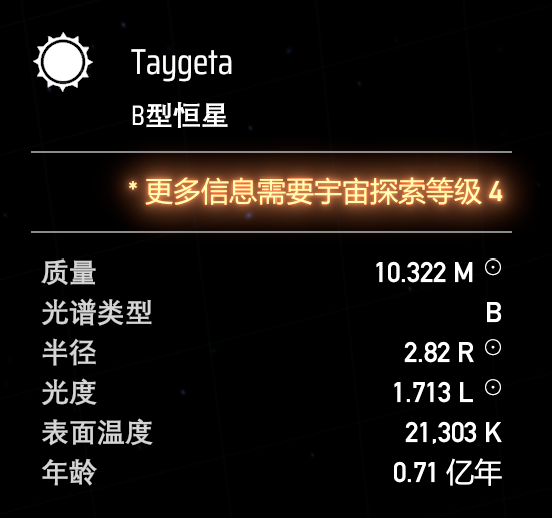
\includegraphics[width=3.5cm]{imgs/screenshots/spheres-info.png}
}及轨道参数。\index{星图}

\section{元数据}

\index{元数据}

0.9.25.11985版本中加入了元数据的设定,每个存档中生产的各种超级矩阵按照每分钟产量分配至元数据中,在其他存档中可以直接提取为超级矩阵或用于研发科技。但若两个存档的星系种子、恒星数量与星球资源倍率完全相同,则\textbf{无法}从该存档中提取元数据。

在创建存档时,设定的星球资源倍率会影响元数据的产出比率,星球的资源倍率越低,单位产量对应的元数据越多。

\begin{table}
    \footnotesize
    \centering
    \caption{行星网格结构}
    \label{tbl:metadata-ratio}
    \begin{tabular}{*{11}{c}}
        \toprule
        资源倍率 & 极少 & 0.5x & 0.8x & 1x & 1.5x & 2x & 3x & 5x & 8x & 无限 \\
        \midrule
        元数据比率 & $400\%$ & $200\%$ & $150\%$ & $100\%$ & $90\%$ & $80\%$ & $70\%$ & $60\%$ & $50\%$ & $40\%$ \\
        \bottomrule
    \end{tabular}
\end{table}